
\documentclass[margin=5mm]{standalone}
\usepackage[T1]{fontenc}
\usepackage[utf8]{inputenc}
\usepackage{pgf,tikz}

\begin{document}

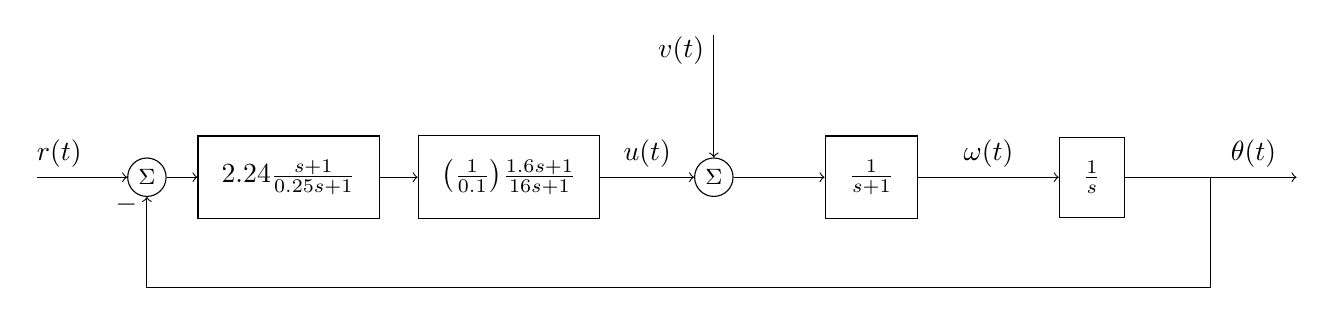
\begin{tikzpicture}[node distance=28mm, anchor=north]
  \node[coordinate] (input) {};
  \node[circle, draw, inner sep=2pt, right of=input, node distance=14mm,] (sum) {\footnotesize $\Sigma$};
   \node[rectangle, draw, right of=sum, inner sep=3mm, node distance=18mm,] (lti) {$2.24\frac{s + 1}{0.25s + 1}$};
   \node[rectangle, draw, right of=lti, inner sep=3mm,] (lag) {$\big(\frac{1}{0.1}\big)\frac{1.6s + 1}{16s + 1}$};
  \node[circle, draw, inner sep=2pt, right of=lag, node distance=26mm,] (sumd) {\footnotesize $\Sigma$};
   \node[rectangle, draw, right of=sumd, inner sep=3mm, node distance=20mm] (lti2) {$\frac{1}{s+1}$};
   \node[rectangle, draw, right of=lti2, inner sep=3mm] (lti3) {$\frac{1}{s}$};
   \node[coordinate, right of=lti3, node distance=26mm] (output) {};
   \node[coordinate, above of=sumd, node distance=18mm] (dist) {};
   \draw[->] (input) -- node[near start, above] {$r(t)$}  (sum);
   \draw[->] (sum) -- node[near start, above] {}  (lti);
   \draw[->] (lti) -- node[near start, above] {}  (lag);
   \draw[->] (lag) -- node[ above] {$u(t)$}  (sumd);
   \draw[->] (dist) -- node[left, very near start] {$v(t)$}  (sumd);
   \draw[->] (sumd) -- node[ above] {}  (lti2);
   \draw[->] (lti2) -- node[ above] {$\omega(t)$}  (lti3);
   \draw[->] (lti3) -- node[coordinate] (meas) {} node[near end, above] {$\theta(t)$} (output);
   \draw[->] (meas) -- ++(0, -14mm) -| node[left, pos=0.96] {$-$} (sum);
 \end{tikzpicture}
\end{document}
